I vores program er der 3 forskellige tærskelværdier som påvirker hvordan
metoden analysere billedet. Marginens brede, afvigelsen af farven i
floodfill og afvigelsen i farven i kandtdetectionen. Alle 3 tærskelværdier er
blevet introduceret i deres respektive afsnit, men ingen konkrate tal
er opgivet. I dette afsnit vil vi opgive de tal, samt en forklaring på
hvorfor vi har valt lige de tal.

\subsection{Marginens brede}
Vi regner marginens brede, $MB$ ud fra en procent af billedets brede og
højde. I afsnittet \ref{opdeling_af_billeder.tex} kom vi frem til en
usikkerhed på $2.1 \%$. Så vores $MB$ skal mindst
være på $2.1 \%$. Ud over det er den minimale forskel på 2 snit vi foretager os,
forskellen mellem det gyldne snit og $\frac{2}{3}$, som vi udregnet i
sektion \ref{opdeling_af_billeder.tex} til maksimalt at have en $MB$ på
$2.43$, for at margin ikke krydser. Så $MB \in [2.1, 2.43]$. Vi har valt
at sætte $MB = 2.4$, da vi derved kan tage højde for uforresette
usikkerhed. XXX(er det en dog nok forklaring).

\subsection{Afvigelsen af farver i kandtdetection}
Det vi bruger kandtdetection til, er af finde en kanter rundt om de
regioner som vi mener er interessante, og undgå de kanter som ligger
inde i regioner. Begge de 2 mål kan ikke altid opfyldes, men vi kan
komme så tæt på et krompromi mellem en perfekt kant rund om region og
ingen kanter inde i region som mulige. Dette gøres ved at ændre 2
tærskelværdier i kantdetectionen ud for observationer som vi har taget
på billederne i forvejen. Vi har valt at dele billederne som vi
observere op i 9 kategorier, som kan ses i tabel
\ref{thressholdsTabelKant}, Kategorier er en grove opdeling af
billederne efter detaljer og farve intensitet, som bruges til at give en
bedre indblik på billedets opbygning. 

\subsubsection{Sammenligninger}
Vi har set på XX(hvor mange) antal malerier og har fundet de
tærskelværdier som vi mener passer bæst på billedet. Vi vil illustrerer
den fremgange måden vi har brugt til at finde tærskelværdierne på, på
maleriet \ref{kDetalier}. Maleriet er malet med mange farver og med
masser af detaljer. Vi ser først på tærskelværdierne
$[0,0],[100,100]......[900,900],[1000,1000]$ se figur \ref{allesammen1}
og \ref{allesammen2}, og finde det interval hvor malerriet ikke har
mistet nogle af kanterne rundt om regionerne i nu, men vil det, i næste
interval. I illustration vurdere vi det til billedet \ref{300-300}, da
billedet \ref{400-400} har mistet for mange af de kanter, som vi gerne
vil beholde. Så tærskelværdien som vi gerne vil finde frem til, befinder
sig fra $[300,300]$ og frem. Ved at sætte den anden tærskelværdig op
lidt af gangen kan vi igen få en række billeder at vælge imellem, for at
få det beste resultat, se sammenligningen i figur \ref{allesammen3}. som
man kan se begynder det er være svær at skelne figurene i \ref{300-850}
og der er lidt for mange kanter i \ref{300-700}, så vi har valt at bruge
tærskeværdigerne $[300,750]$ for dette billedet. Man kunne god gå længer
ned og se om tærskeværdig $[300,745]$ passet bedre, men vi har valt at
holde . Det maleri vi lige har brugt er ikke særlige repræsentativ for
helle vores maleri database, så vi har taget en række billeder og brugt
samme metode på dem og kommer frem til en middel tærskelværdi, jeg viser
her en lille udsnit af dem, se figur \ref{en},\ref{to},\ref{the}

\begin{figure}[!h]
    \centering
    \subfloat[100,100]{
        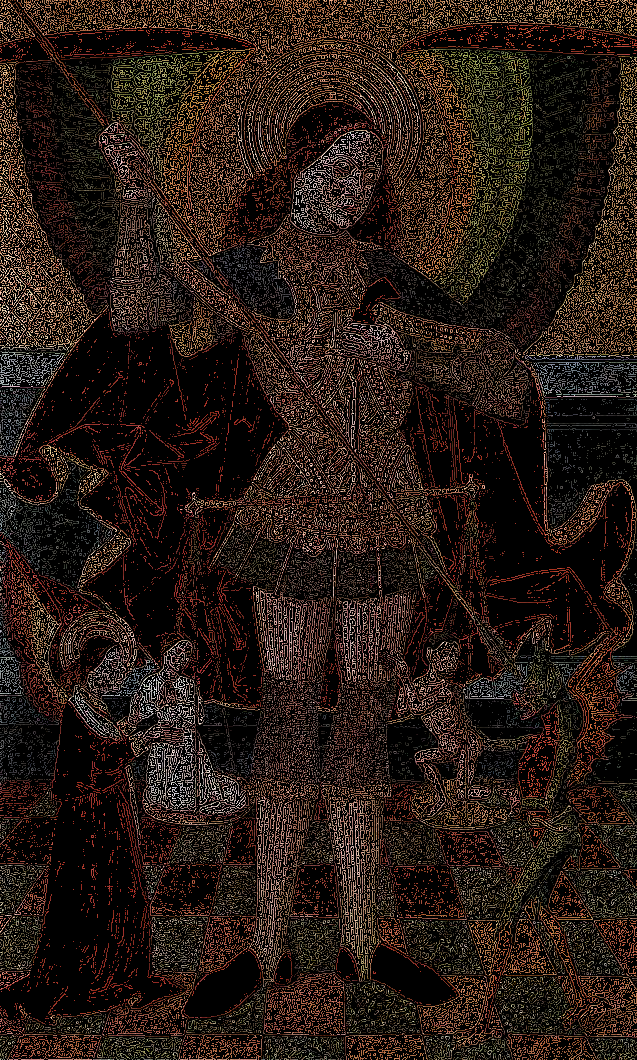
\includegraphics[angle=0,width=0.45\textwidth]{afsnit/afprovning/billeder/thressholds/krafitige_farver/krafite_detalier/1_iteration/100-100.png}
        \label{100-100}}\hspace{1em}
    \subfloat[200,200]{
        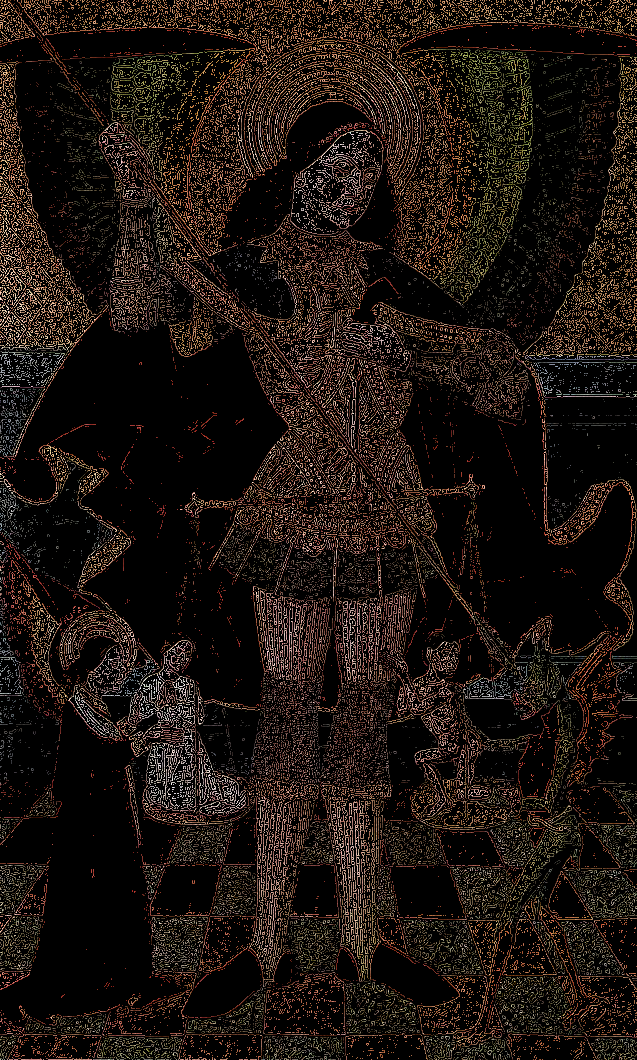
\includegraphics[angle=0,width=0.45\textwidth]{afsnit/afprovning/billeder/thressholds/krafitige_farver/krafite_detalier/1_iteration/200-200.png}
        \label{200-200}}\\
    \subfloat[300,300]{
        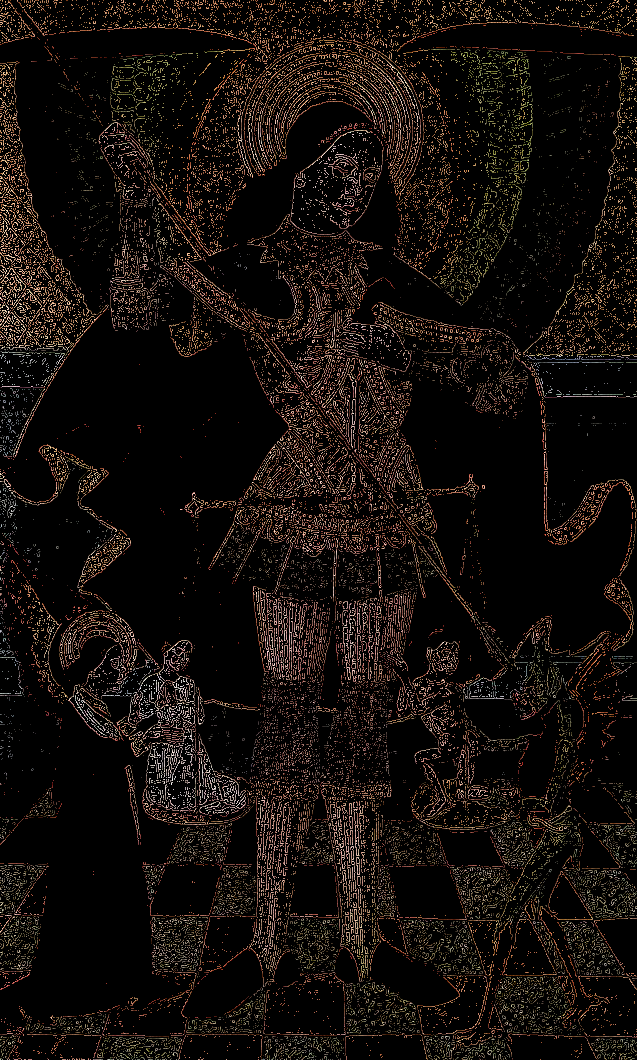
\includegraphics[angle=0,width=0.45\textwidth]{afsnit/afprovning/billeder/thressholds/krafitige_farver/krafite_detalier/1_iteration/300-300.png}
        \label{300-300}}\hspace{1em}
    \subfloat[400,400]{
        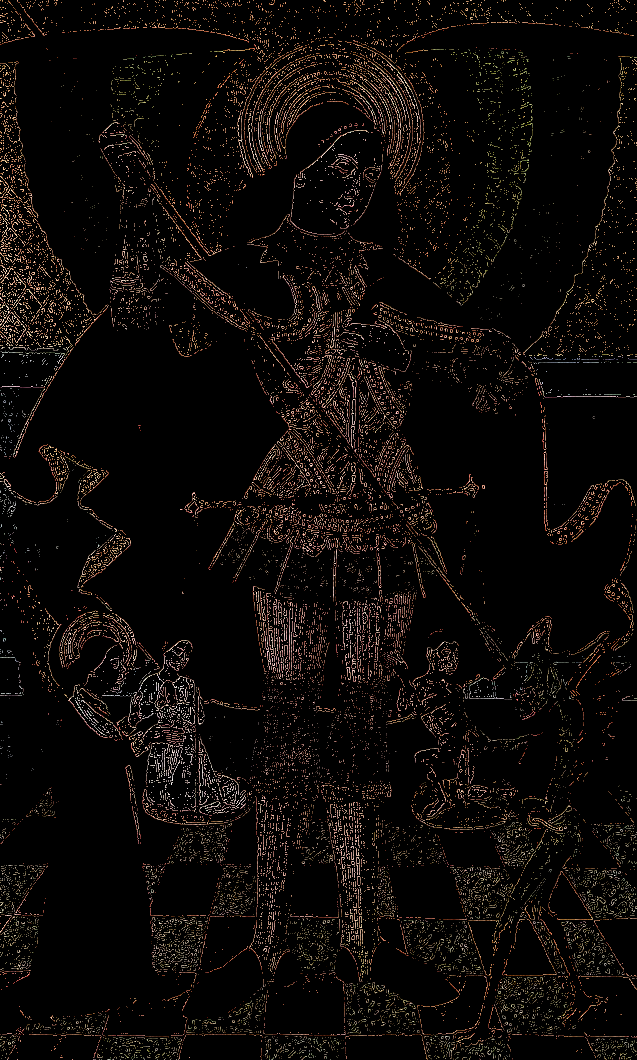
\includegraphics[angle=0,width=0.45\textwidth]{afsnit/afprovning/billeder/thressholds/krafitige_farver/krafite_detalier/1_iteration/400-400.png}
        \label{400-400}}\\
     \label{allesammen1}
\end{figure}

\begin{figure}[!h]
	\centering
	\subfloat[500,500]{
        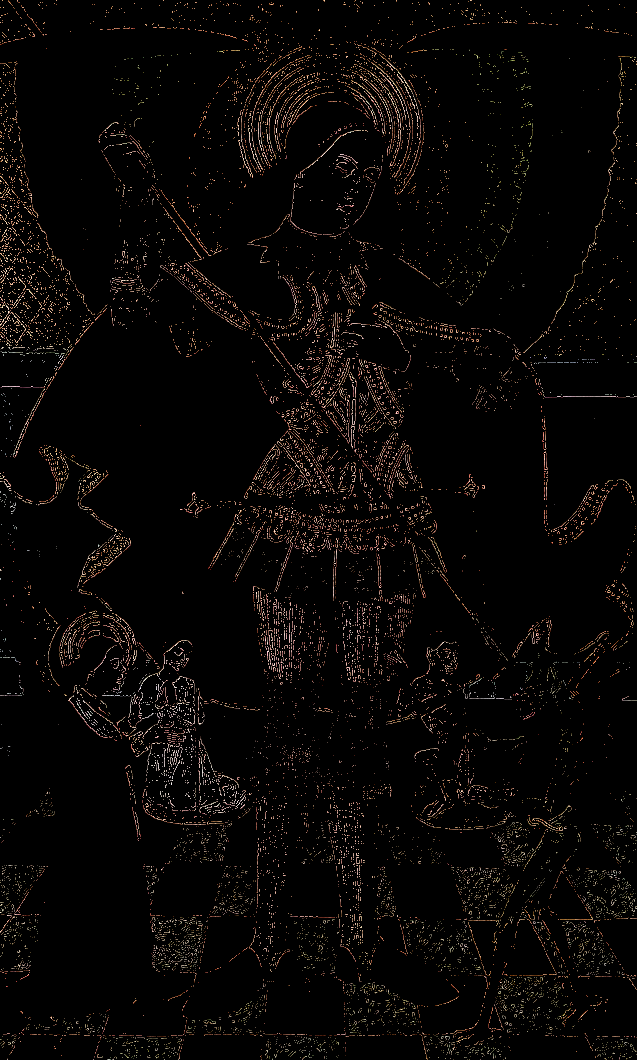
\includegraphics[angle=0,width=0.45\textwidth]{afsnit/afprovning/billeder/thressholds/krafitige_farver/krafite_detalier/1_iteration/500-500.png}
        \label{500-500}}\hspace{1em}
    \subfloat[600,600]{
        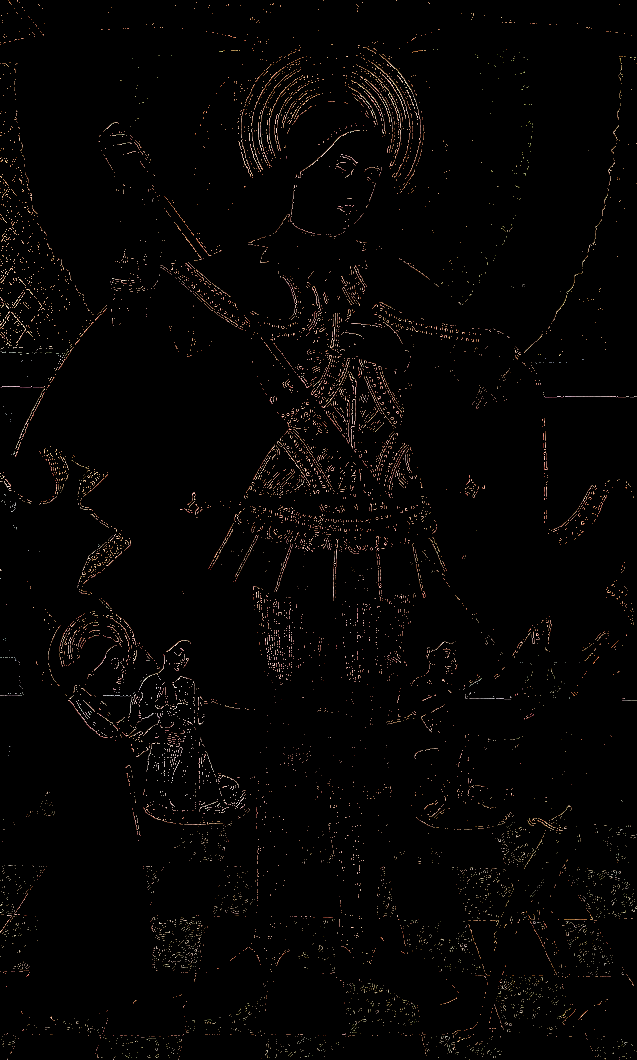
\includegraphics[angle=0,width=0.45\textwidth]{afsnit/afprovning/billeder/thressholds/krafitige_farver/krafite_detalier/1_iteration/600-600.png}
        \label{600-600}}\\
    \subfloat[700,700]{
        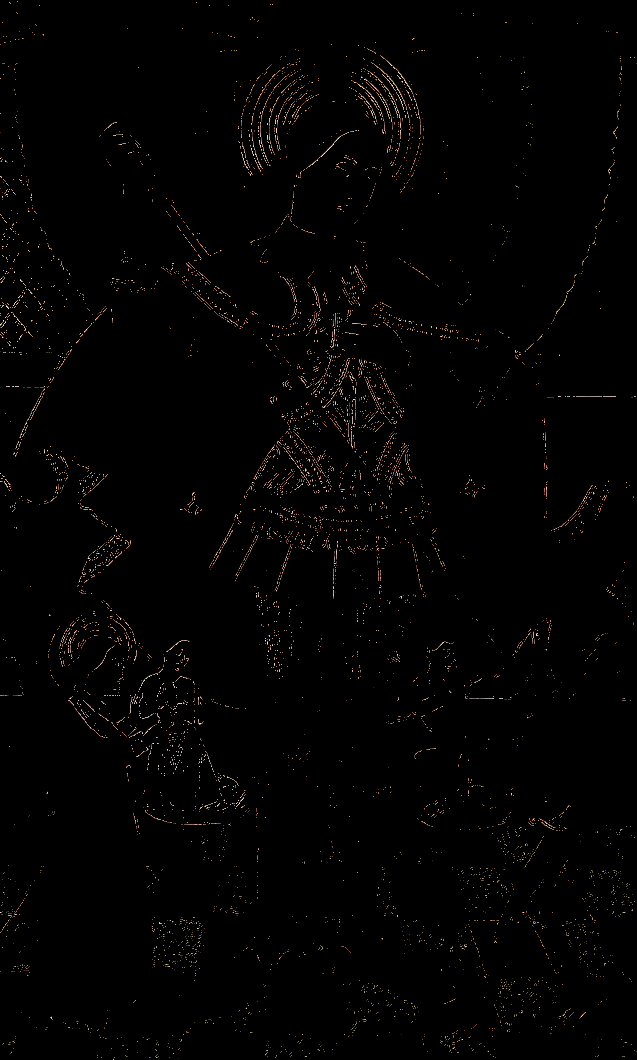
\includegraphics[angle=0,width=0.45\textwidth]{afsnit/afprovning/billeder/thressholds/krafitige_farver/krafite_detalier/1_iteration/700-700.png}
        \label{700-700}}\hspace{1em}
    \subfloat[Original]{
        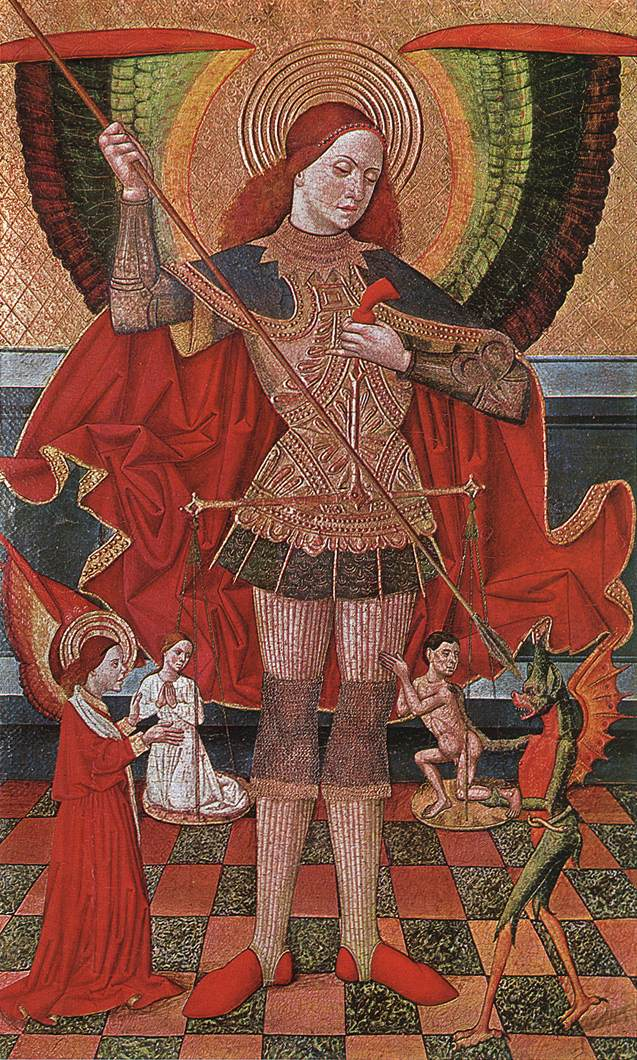
\includegraphics[angle=0,width=0.45\textwidth]{afsnit/afprovning/billeder/thressholds/krafitige_farver/krafite_detalier/kDetalier.jpg}
        \label{kDetalier}}\\
    \caption[]{Edgedetection på maleriet \ref{kDetalier} som har mange detaliger og kraftige farver, med tærskelværdierne fra 100-100 til 700-700}
     \label{allesammen2}
\end{figure}

\begin{figure}[!h]
    \centering
    \subfloat[300,700]{
        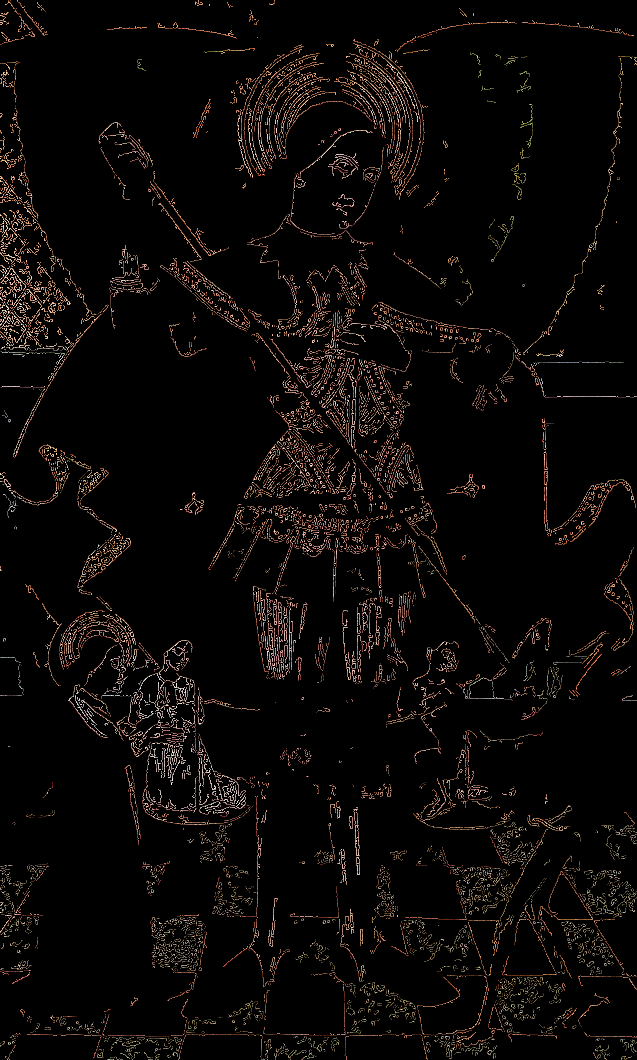
\includegraphics[angle=0,width=0.45\textwidth]{afsnit/afprovning/billeder/thressholds/krafitige_farver/krafite_detalier/2_iteration/300-700.png}
        \label{300-700}}\hspace{1em}
    \subfloat[300,750]{
        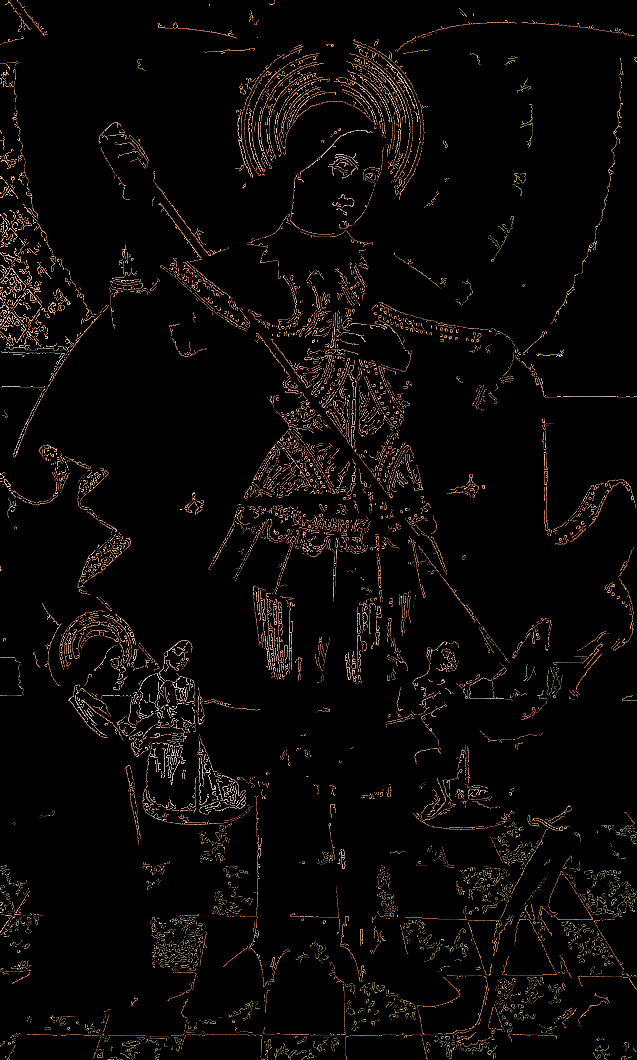
\includegraphics[angle=0,width=0.45\textwidth]{afsnit/afprovning/billeder/thressholds/krafitige_farver/krafite_detalier/2_iteration/300-750.png}
        \label{300-750}}\\
    \subfloat[300,800]{
        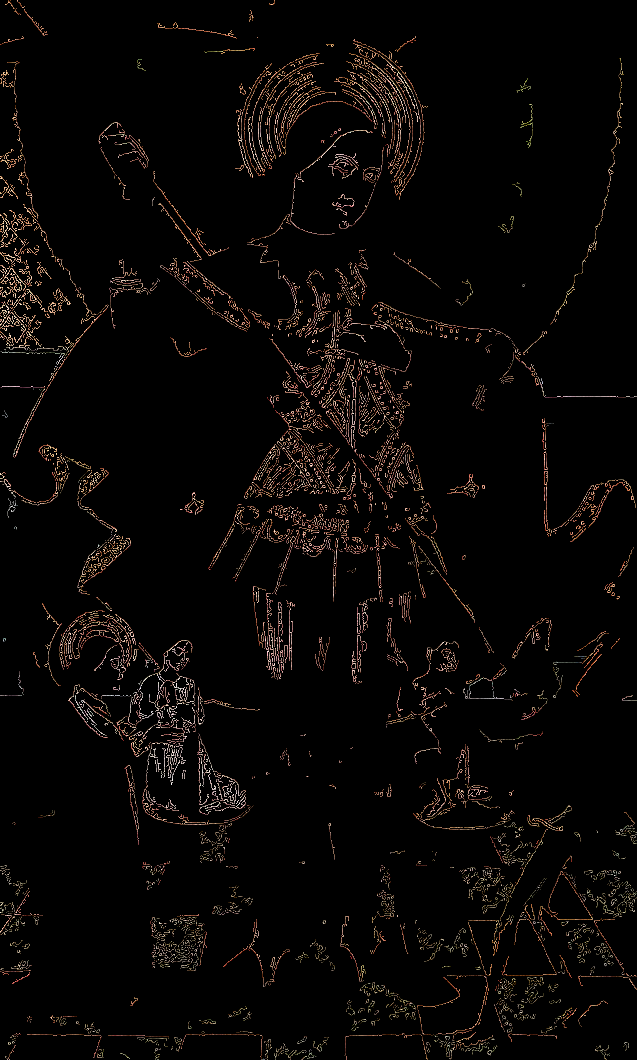
\includegraphics[angle=0,width=0.45\textwidth]{afsnit/afprovning/billeder/thressholds/krafitige_farver/krafite_detalier/2_iteration/300-800.png}
        \label{300-800}}\hspace{1em}
    \subfloat[300,850]{
        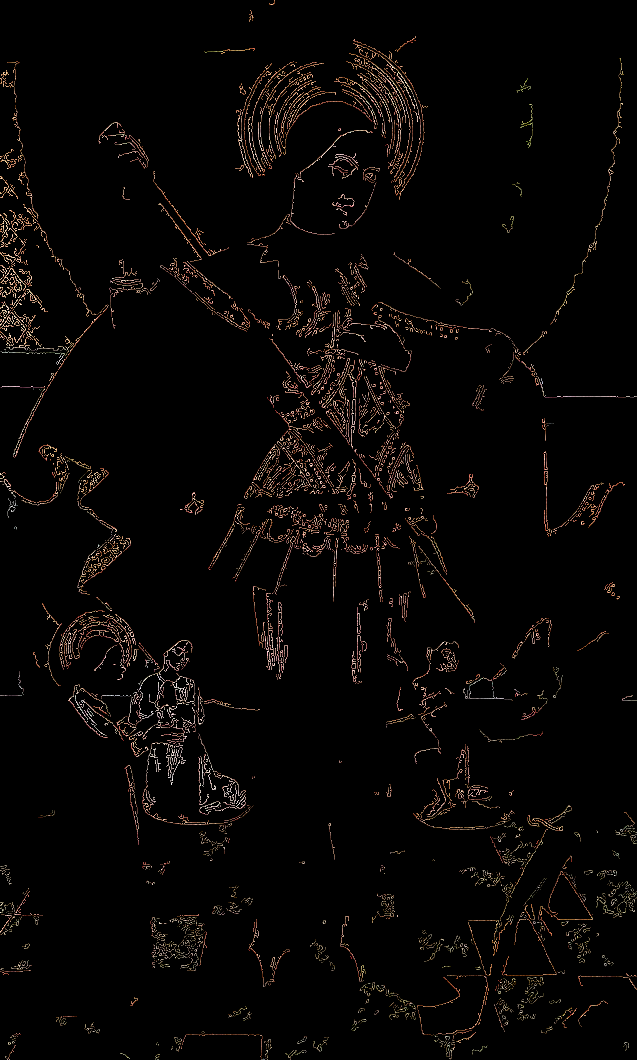
\includegraphics[angle=0,width=0.45\textwidth]{afsnit/afprovning/billeder/thressholds/krafitige_farver/krafite_detalier/2_iteration/300-850.png}
        \label{300-850}}\\
        \caption[]{Edgedetection hvor de 4 billeder som er intrasante taget med}
     \label{allesammen3}
\end{figure}
 
\begin{figure}[!h]
    \centering
    \subfloat[100,250]{
        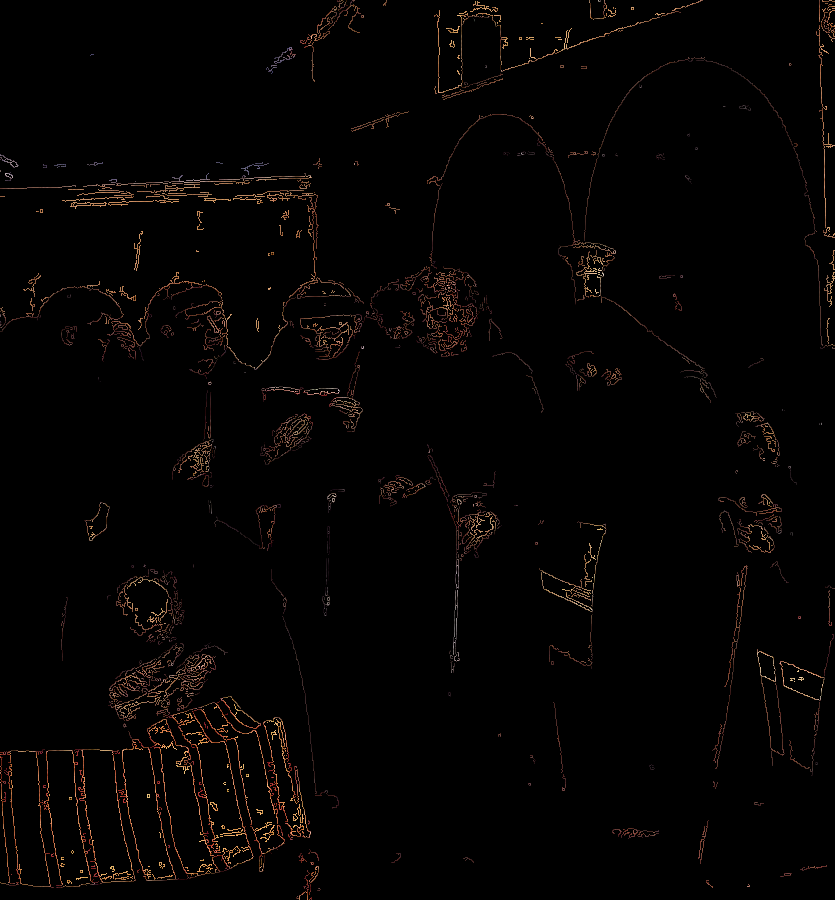
\includegraphics[angle=0,width=0.45\textwidth]{afsnit/afprovning/billeder/thressholds/svage_farver/svage_detalier/2_iteration/100-250.png}
        \label{100-250}}\hspace{1em}
    \subfloat[Orginal]{
        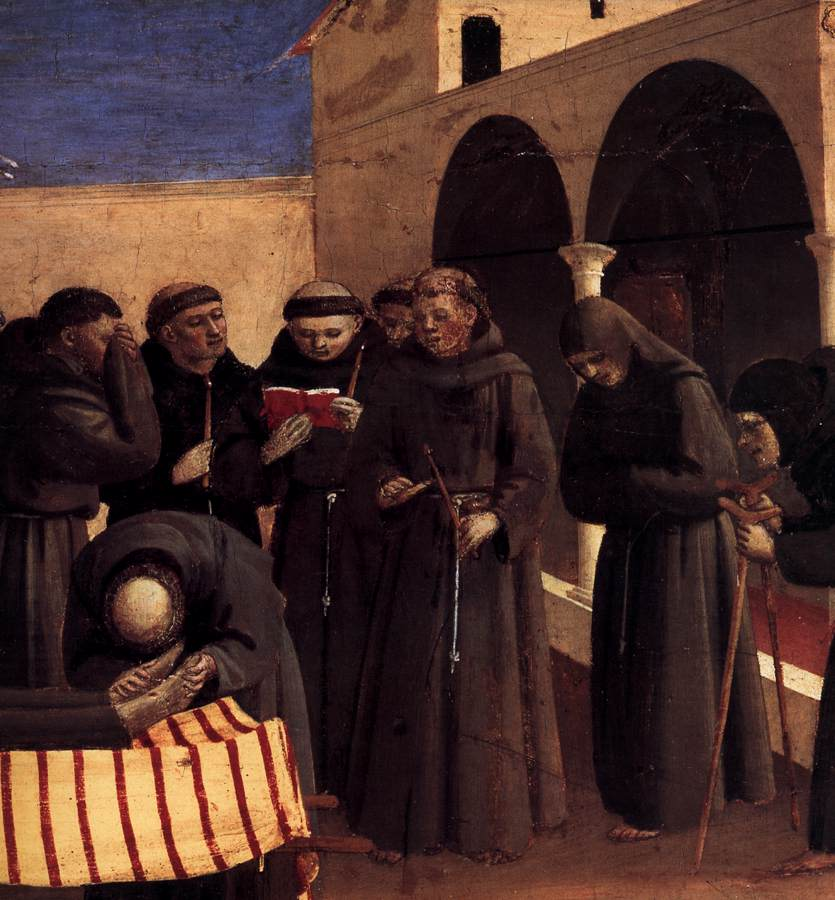
\includegraphics[angle=0,width=0.45\textwidth]{afsnit/afprovning/billeder/thressholds/svage_farver/svage_detalier/sDetalier.jpg}
        \label{Orginal}}\\
        \caption[]{Edgedetection på et billedet med svage farver og få detalier, hvor tærskenværdigern [100,250] er den beste}
     \label{en}
\end{figure}

\begin{figure}[!h]
    \centering
    \subfloat[100,240]{
        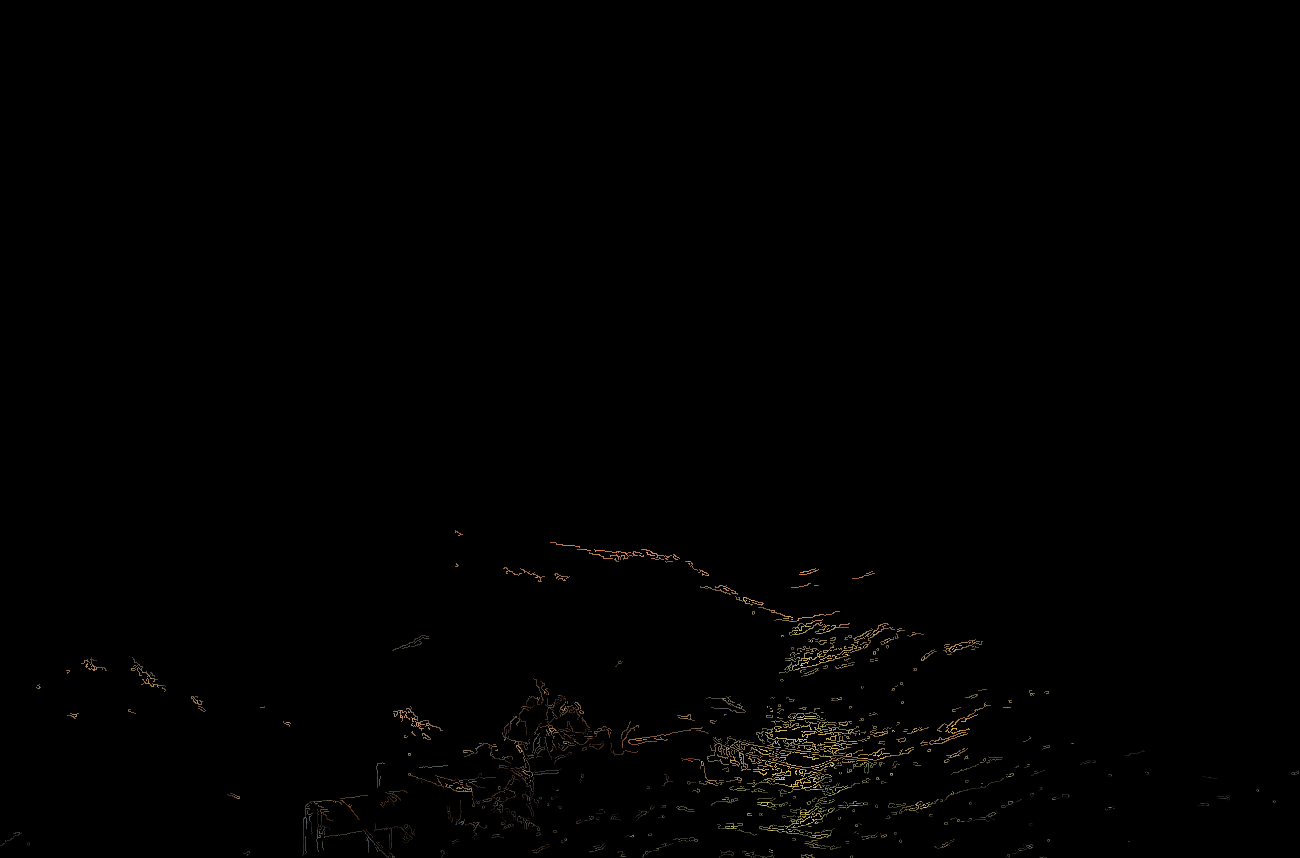
\includegraphics[angle=0,width=0.45\textwidth]{afsnit/afprovning/billeder/thressholds/medium_farver/svage_detalier/2_iteration/100-240.png}
        \label{100-240}}\\
    \subfloat[Orginal]{
        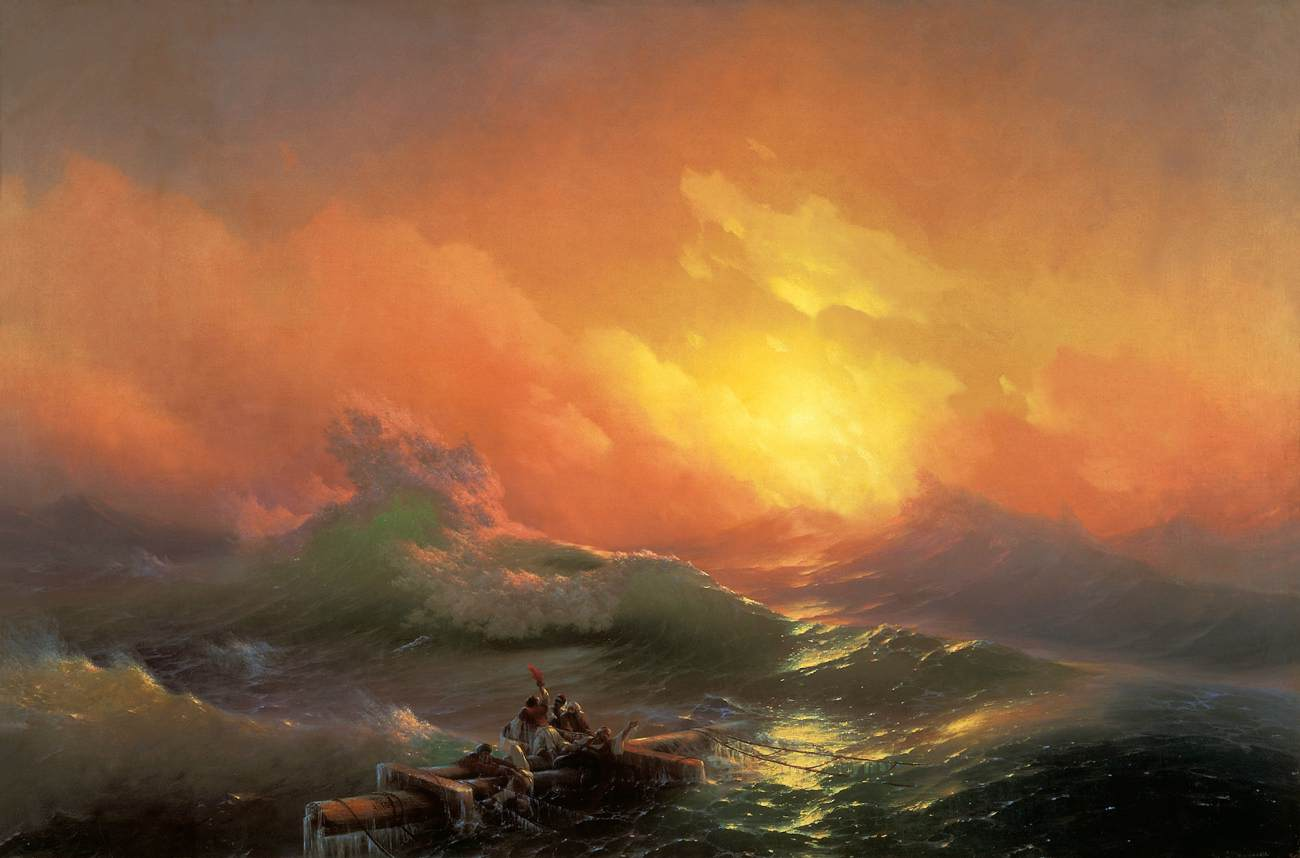
\includegraphics[angle=0,width=0.45\textwidth]{afsnit/afprovning/billeder/thressholds/medium_farver/svage_detalier/sDetalier1.jpg}
        \label{Orginal}}\\
        \caption[]{Edgedetection på et billedet med medium farver og få detalier, hvor tærskenværdigern [100,240] er den beste}
     \label{to}
\end{figure}

\begin{figure}[!h]
    \centering
    \subfloat[200,460]{
        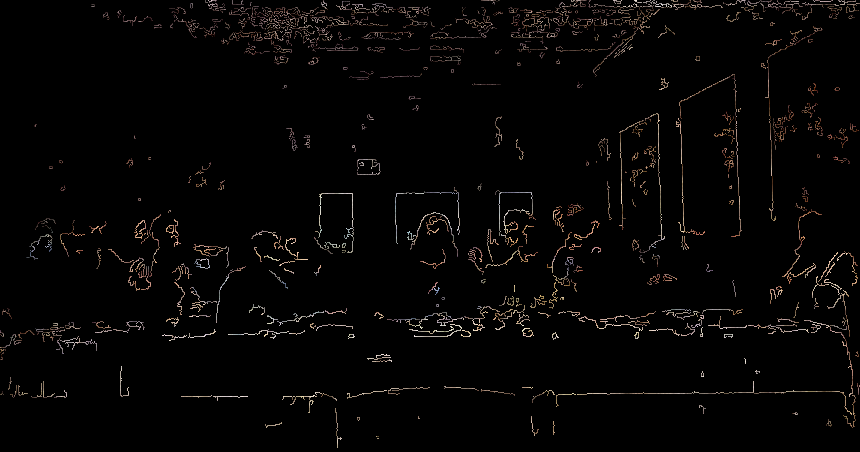
\includegraphics[angle=0,width=0.45\textwidth]{afsnit/afprovning/billeder/thressholds/medium_farver/medium_detalier/2_iteration/200-460.png}
        \label{200-460}}\\
    \subfloat[Orginal]{
        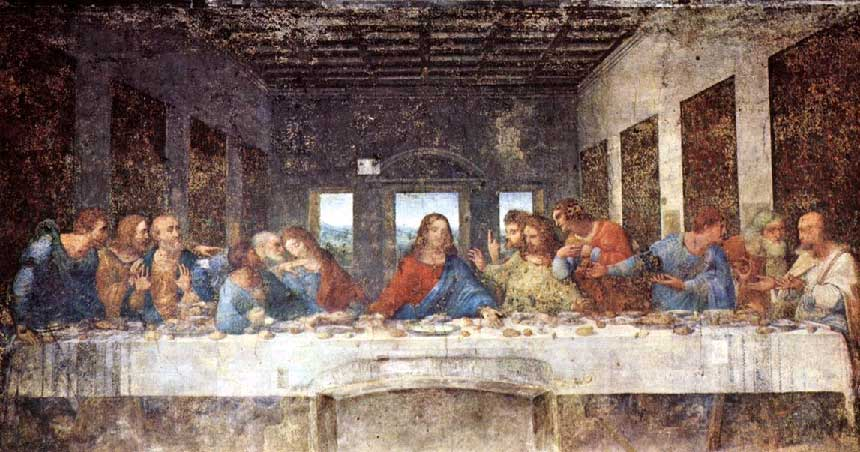
\includegraphics[angle=0,width=0.45\textwidth]{afsnit/afprovning/billeder/thressholds/medium_farver/medium_detalier/mDetalier1.jpg}
        \label{Orginal}}\\
        \caption[]{Edgedetection på et billedet med medium farver og medium detalier, hvor tærskenværdigern [200,460] er den beste}
     \label{tre}
\end{figure}

\begin{tabular}{| l | l | l | l |} \hline
  						& Svage farver 	& Medium farver & kraftige farver \\ \hline
	Få detalier 		& [100,250]		& [100,240]		& [200,320]\\ \hline
	Medium detalier 	& [100,280]		& [200,460]		& [200,380]\\ \hline
	Mange detalier		& [200,400]		& [200,380]		& [300,750]\\ \hline
\end{tabular} \label{thressholdsTabelKant}

Som man kan se at tabel \ref{thressholdsTabelKant} gå tærskelværdierne
fra [100,240] til [300,750], så vi kan ikke umiddelbart sætte en fast
tærskelværdi for alle malerier og få at lave en rigtige undersøgelse af
tærskelværdi på malerierne, bliver man nød til at se på mangle flere
malerierne og bestemme deres tærskelværdi og udregne median af de
værdiger, men det vil krave en støre undersøgelse som vi ikke har valt
at gøre, af 3 grunde. 1, det vil kun være en median tærskelværdi få lige
det sæt malerier som vi arbejder på. 2 det vil krave at vi gennemgik
XX(hvor mange) billeder. 3, selv med en median tærskelværdi vil der
stadig være en stor rigge malerier hvor median tærskelværdien ikke vil
være særlige god for. En anden fremgang måde er at regne
tærskelværdierne løbene ud for vært billedet via et program. Men det
problem falder uden for denne opgave og vi vil derfor ikke komme ind på
det. Selv om vi måske ikke kan få det vi helst vil have er der stadig en
del observationer som kan laves ud fra tabellen
\ref{thressholdsTabelKant}. Tærskelværdierne bliver højre nu flere
detaljer og nu kraftigere farverne er. Det virker også som om mange
detaljer vægter lige højt i forholdt til tærskelværdierne en kraftige
farver. Den anden tærskelværdi er ca 2.5 gangen støre en den første
tærskelværdi.\\

De tærskelværdier som vi har fundet svare til de optimale
tærskelværdier for maleriet, men vi kan godt bruge en værdig som ligger
laver, da metoden floodfill som gør brug af kandtdetektionen resultatset,
god kan tage højde for små kanter, men fejler hvis der ikke er nogle.
Derfor har vi valt at bruger den nederste tærskelværdi som vi har fundet
[100,240] og sænke den lidt til $[78,78 \cdot 2.5 ]$.

\subsection{Afvigelsen af farver i floodfill}
Floodfill har 2 tærskelværdier $lo$ og $up$, som betegner hvor mange
pixel værdier en nabo pixel farver må variere ned og op, en fyldestgørelses
beskrivelse af floodfill findes i afsnit \ref{floodfill}. Vi har tænkt
os at finde en fældes tærskelværdi til brug i vores program. Måde vi gør
det på at ved at observere hvordan floodfill virker med forskellige
tærskelværdier og finde de tærskelværdier som passer bæst til
maleriet. Resultatet for observationen kan ses i tabel \ref{thressholdsTabelFF}, hvor de 9 sammen kategorier er vist. Et af de malerierne hvor den optimale tærskelværdi er fundet se i figur \ref{Floodfillbilledet}, så man kan se hvad vi har vurderet til at være den beste værdi.

\begin{figure}[!h]
    \centering
    \subfloat[8,8]{
        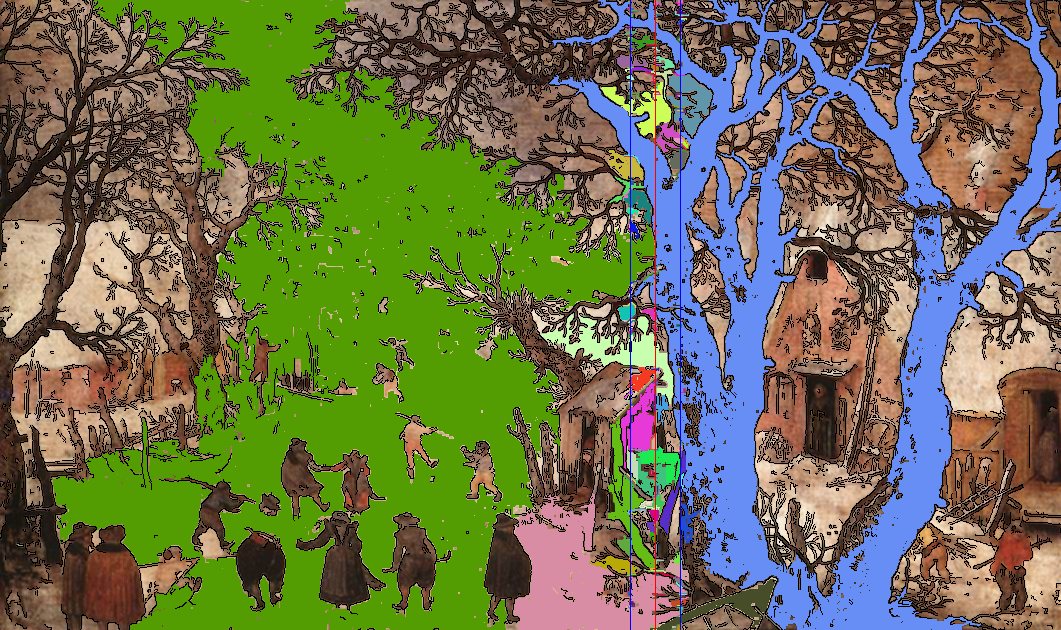
\includegraphics[angle=0,width=0.9\textwidth]{afsnit/afprovning/billeder/thressholds/svage_farver/kraftige_detalier/floodfill/8-8.png}
        \label{8-8}}\\
    \subfloat[Orginal]{
        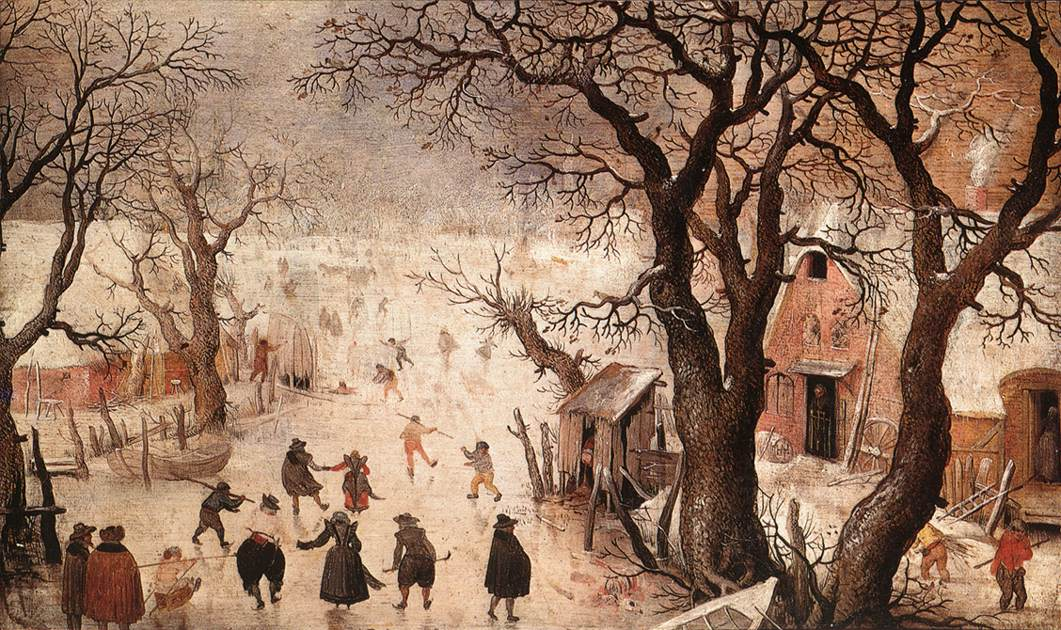
\includegraphics[angle=0,width=0.9\textwidth]{afsnit/afprovning/billeder/thressholds/svage_farver/kraftige_detalier/kDetalier.jpg}
        \label{Orginal}}\\
        \caption[]{tærskelværdierne på et billedet med svage farver og kraftige detaljer hvor tærskelværdien [8,8] passer best}
     \label{Floodfillbilledet}
\end{figure}

\begin{tabular}{| l | l | l | l |} \hline
  						& Svage farver 		& Medium farver & kraftige farver \\ \hline
	Få detalier 		& \textbf{[2,2]}	& [3,3]			& [4,4]\\ \hline
	Medium detalier 	& \textbf{[2,2]}	& \textbf{[5,5]}& \textbf{[2,2]}\\ \hline
	Mange detalier		& [8,8]				& [4,4]			& [7,7]\\ \hline
\end{tabular} \label{thressholdsTabelFF}\\\\

Som man kan af tabellen er nogle af vadierne med fed, begrundelsen for det er at de vadier er de beste vi kunne finde for billedet, men at de vadier stadig ikke giver noget som er særlige brugbart, se sektion \ref{floodfilltest}. værdigerne i tabel fluktuere også en del, så vi har igen samme problem stilling som i tærskelværdierne ved kantdetektion og har valt at bruge tærskelværdien [4,4] da dette kommer tættest på gennemsnit.
